\documentclass[10pt,t]{beamer}
\usepackage{msvcommon}

%Imported from Thesis Report

\usepackage{amssymb}
\usepackage{amsmath}
\usepackage{float}
\usepackage{subfig}
\usepackage[titletoc]{appendix}
\usepackage{siunitx}

\usepackage{eurosym}
\usepackage{listings,cprotect}
\usepackage{soul,xcolor}\lstset{escapeinside={(*@}{@*)}}

% User defined Listing
\lstdefinestyle{DOS}
{
    backgroundcolor=\color{white},
    basicstyle=\scriptsize\color{black}\ttfamily
}

\usepackage{hyperref}
\usepackage{pdfpages}
\usepackage{rotating}
\usepackage{pdflscape}

%\usepackage[style=verbose-ibid,backend=bibtex]{biblatex}
%\usepackage{bibentry}

% Packages for Jonas Maas's Thesis Tikz block diagrams
\usepackage{tikz}
\usetikzlibrary{arrows.meta, calc}
\newcommand{\B}[1]{\boldsymbol{#1}}
\newcommand{\Bhat}[1]{\boldsymbol{\hat{#1}}}
\newcommand{\e}[1]{\emph{#1}}

\usepackage{caption}

% -------------------------------------------------------------------------------
% ** Input Encoding
% - utf8x is recommended at MSV
% - Some comments on encoding can be found here:
%   https://groups.google.com/forum/?fromgroups=#!msg/comp.text.tex/4LC-xODb-LU/1Bd5UZOMNM4J
%
\ifxetexorluatex
  % XeTeX and LuaTeX support utf8 by default
\else
  % File encoding utf8x
  %\usepackage{ucs}
  %\usepackage[utf8x]{inputenc}
  \usepackage[utf8]{inputenc}
\fi
%
%--------------------------------------------------------------------------------
% ** Language Settings and Hyphenation Patterns
%
% Note: final argument to babel sets the main language
%
\ifxetex%
\usepackage{polyglossia}
  \setmainlanguage{english}
  \setotherlanguage{german}
\else
  \usepackage[ngerman,english]{babel}
\fi

% Custom defines
\usepackage{bbding}
\newcommand*\tick{\item[\textcolor{green}{\Checkmark}]}
\newcommand*\fail{\item[\textcolor{red}{\XSolidBrush}]}


%--------------------------------------------------------------------------------
% ** MSV style defintions for beamer presentations
%
\usepackage[colorblock]{msvpresentation}
%-------------------------------------------------------------------------------
% ** Options for msvpresentation (all options are disabled by default)
% 1) boolean options for msvpresentation package:
%  | bw             | black and white color scheme                             |
%  | colorblock     | use non-white background colors for blocks               |
%  | frameblock     | use colored borders for blocks                           |
%
%--------------------------------------------------------------------------------
% ** Setup look of presentation
%
% MSV style should be compatible with the beamer themes
%
\useinnertheme{default}
\useoutertheme{default}

% Colors:
%\usecolortheme[named=TUMDarkerBlue]{structure} % variant: TUMBlack
\usecolortheme[named=TUMBlack]{structure} % variant: TUMBlack
\setbeamercolor{frametitle}{fg=TUMBlack} % variant: TUMDarkerBlue
\setbeamercolor{normal text}{fg=TUMBlack,bg=TUMWhite} % font/background
\setbeamercolor{alerted text}{fg=TUMBeamerRed,bg=TUMWhite} % alert boxes
\setbeamercolor{example text}{fg=TUMBeamerGreen,bg=TUMWhite} % example boxes

% Headers, Footers, Titlepage:
%   Note: can adjust height of the frame title with \raisetitle and \lowertitle
\setbeamertemplate{headline}[tum] % no, tum, msvtum
\setbeamertemplate{footline}[authortitle] % minimal, author, authortitle
\setbeamertemplate{title page}[tum][left] % with clock tower
%\setbeamertemplate{title page}[default][left,sep=0pt] % without clock tower

%--------------------------------------------------------------------------------
% ** Presentation title, author, etc.
%
\title{Experimental Evaluation of Machine Learning based Wireless Communication Algorithms}
\author[Karthik Sukumar (TUM)]{Karthik Sukumar}
\institute{\MSVname}
\date{07. Sep 2020}

\usepackage[style=verbose-ibid,backend=bibtex]{biblatex}
%\usepackage{bibentry}
\addbibresource{../bibfile}

\begin{document}
{

%\bibliographystyle{../IEEEtran}
%\bibliography{../bibfile}

% use custom header/footer for title page
\setbeamertemplate{headline}[tum]
\setbeamertemplate{footline}[no]
\begin{frame}
\titlepage
\end{frame}
}

\section{Introduction}
\subsection{A Typical Slide}

%Intro Page

\begin{frame}{Introduction}

    \begin{itemize}
        \item Channel Estimation is vital for any Wireless systems
            \bigskip
        \item Required to revert the channel propogation effects
            \bigskip
            \pause

        \item For perfect Channel estimation, pilot symbols are to be placed on all sub carriers
            \bigskip
        \item For massive MIMO $\Rightarrow$ No. of Antennas $\propto$ Pilot overhead
            \bigskip
            \pause

        \item Current reseach for potential solutions include
            \begin{itemize}
                \item Model based channel estimation % where a 3D model of the environment is saved and ray tracing is used to find the Channel
                \item Machine learning based algorithms to find the channel
            \end{itemize}
    \end{itemize}

%\bigskip % Use \bigskips between paragraphs (do not set \parskip as this distorts block environments)

\end{frame}

\begin{frame}{Summary of Thesis}
    \begin{itemize}
        \item Setup a MIMO Test Jig
            \bigskip
            \pause
        \item Collect real world experimental Tx-Rx data from the MIMO Setup
            \bigskip
            \pause
        \item Use the data to train a Inverted Neural Network \footnote{Jonas Maas. “Invertible Neural Networks for MIMO Detection”. BA thesis. Technical University of Munich, 2020.} as shown below
            \bigskip
            \bigskip

            \begin{center}
                \begin{figure}[H]
                    \resizebox{8cm}{!}{
                        \begin{tikzpicture}
                            \tikzstyle{network} = [rectangle, draw, minimum height = 15mm, minimum width = 20mm, line width = 0.5mm]

                            \node (a) at (0, 0) {$\Bhat{x}_j$};
                            \node[network] at (3, 0) (b) {Singlestream ML};
                            \node[network] at (7, 0) (c) {$\text{INN}^{-1}$};
                            \node (d) at (11, 0) {$\B{y}_j = \B{Hx}_j + \B{n}_j$};

                            \draw[->, line width = 0.5mm] (d) to (c);
                            \draw[->, line width = 0.5mm] (c) to node [above] {$\Bhat{x}_{\text{estim}, j}$} (b) ;
                            \draw[->, line width = 0.5mm] (b) to (a);

                        \end{tikzpicture}
                    }
                    \caption{ML Model for learning the network}
                    \label{fig:MLModel}
                \end{figure}
            \end{center}


            %\begin{itemize}
            %    \item Machine learning based channel prediction algorithms
            %\end{itemize}
    \end{itemize}
\end{frame}

\begin{frame}{Summary of Thesis}

    \begin{itemize}
        \item Software Defined Radio - USRP
            \bigskip
        \item Possible Options for a MIMO Setup
            \bigskip
        \item LTE Fundamentals
            \bigskip
        \item Chosen Experimental Setup
            \bigskip
        \item Results
            \bigskip
        \item Conclusions and future work
    \end{itemize}
\end{frame}

\begin{frame}{Software Defined Radio - USRP}
    \begin{table}[H]
        \begin{center}
            \resizebox{7cm}{!}{
            \begin{tabular}{|l|c|}
                \hline
                Model                   & USRP2940          \\ \hline
                Baseband Bandwidth      & 40\si{\mega\hertz}             \\ \hline
                RF-Operating Frequency  & 50\si{\mega\hertz}-2200\si{\mega\hertz}     \\ \hline
                FPGA                    & Kintex-7 410T     \\ \hline
                No of Transmitters      & 2                 \\ \hline
                No of Receivers         & 2                 \\ \hline
                Connectivity            & MXIe, Ethernet    \\ \hline
                Oscillator              & Internal Crystal  \\ \hline
                ADC/DAC                 & 14 (For Rx)/16 (For Tx) bit         \\ \hline
                Frequency Accuracy      & 2.5 ppm           \\ \hline
                Maximum Power Output    & 20\si{\dB}\si{\milli}             \\ \hline
                Maximum I/Q Sample Rate & 200\si{\mega\hertz}            \\ \hline
            \end{tabular}
        }
        \end{center}
        \caption{USRP2940 SDR Product details}
        \label{tb:USRP}
    \end{table}
\end{frame}

\begin{frame}{Software Defined Radio - USRP}
    \begin{figure}[H]
        \resizebox{5cm}{!}{
        \centering
        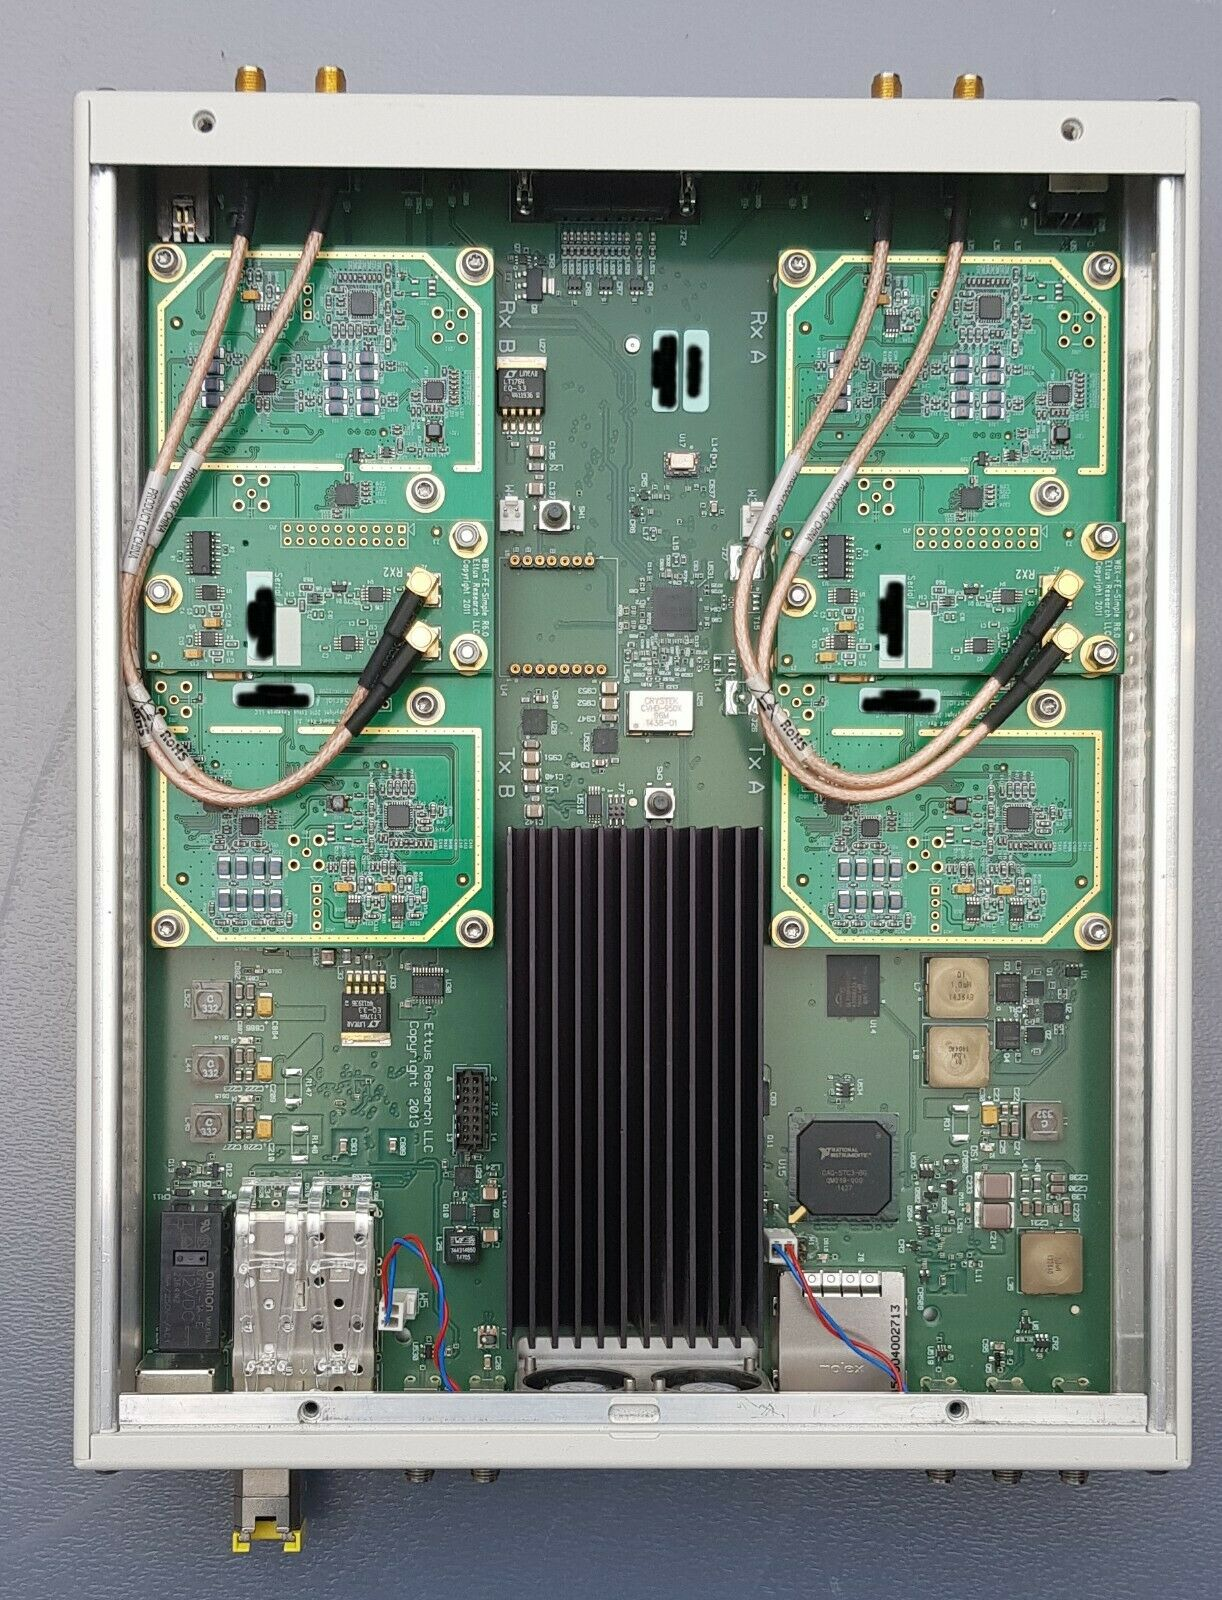
\includegraphics[width=\linewidth]{../images/National-Instruments-USRP-2940R-Ettus-Research-X300.jpg}
    }
        \caption{Insides of USRP2940}
        \label{fig:SyncFail2Ch}%
    \end{figure}
\end{frame}

\begin{frame}{Possible Options for a MIMO Setup}
    \begin{enumerate}
        \item Standalone USRP
            \pause
            \begin{itemize}
                    \tick Minimum Hardware required
                    \tick Modular as long as we could use PCIe expanders
                    \fail Needs the Octoclock a Clock distribution accessory
                    \fail Transceivers not synchronised
            \end{itemize}
            \pause
        \item MIMO Application Framework
            \pause
            \begin{itemize}
                    \tick Modular MIMO setup
                    \tick supports upto 128 Antennas on the BS
                    \fail Expensive$! >$\euro100.000 for a minimum working setup
                    \fail Needs many additional HW components
            \end{itemize}
            \pause
        \item LTE Application Framework
            \pause
            \begin{itemize}
                    \tick Only 2 USRPs and a Host are required
                    \fail Limited to 2x2 MIMO setup
            \end{itemize}
    \end{enumerate}

\end{frame}

\begin{frame}{Option 1 - Standalone USRP}
    \pause
    \begin{center}
        $
        y(t) = cos(\omega{t}) + j*sin(\omega{t})
        $
    \end{center}
    \begin{figure}[H]
        \centering
        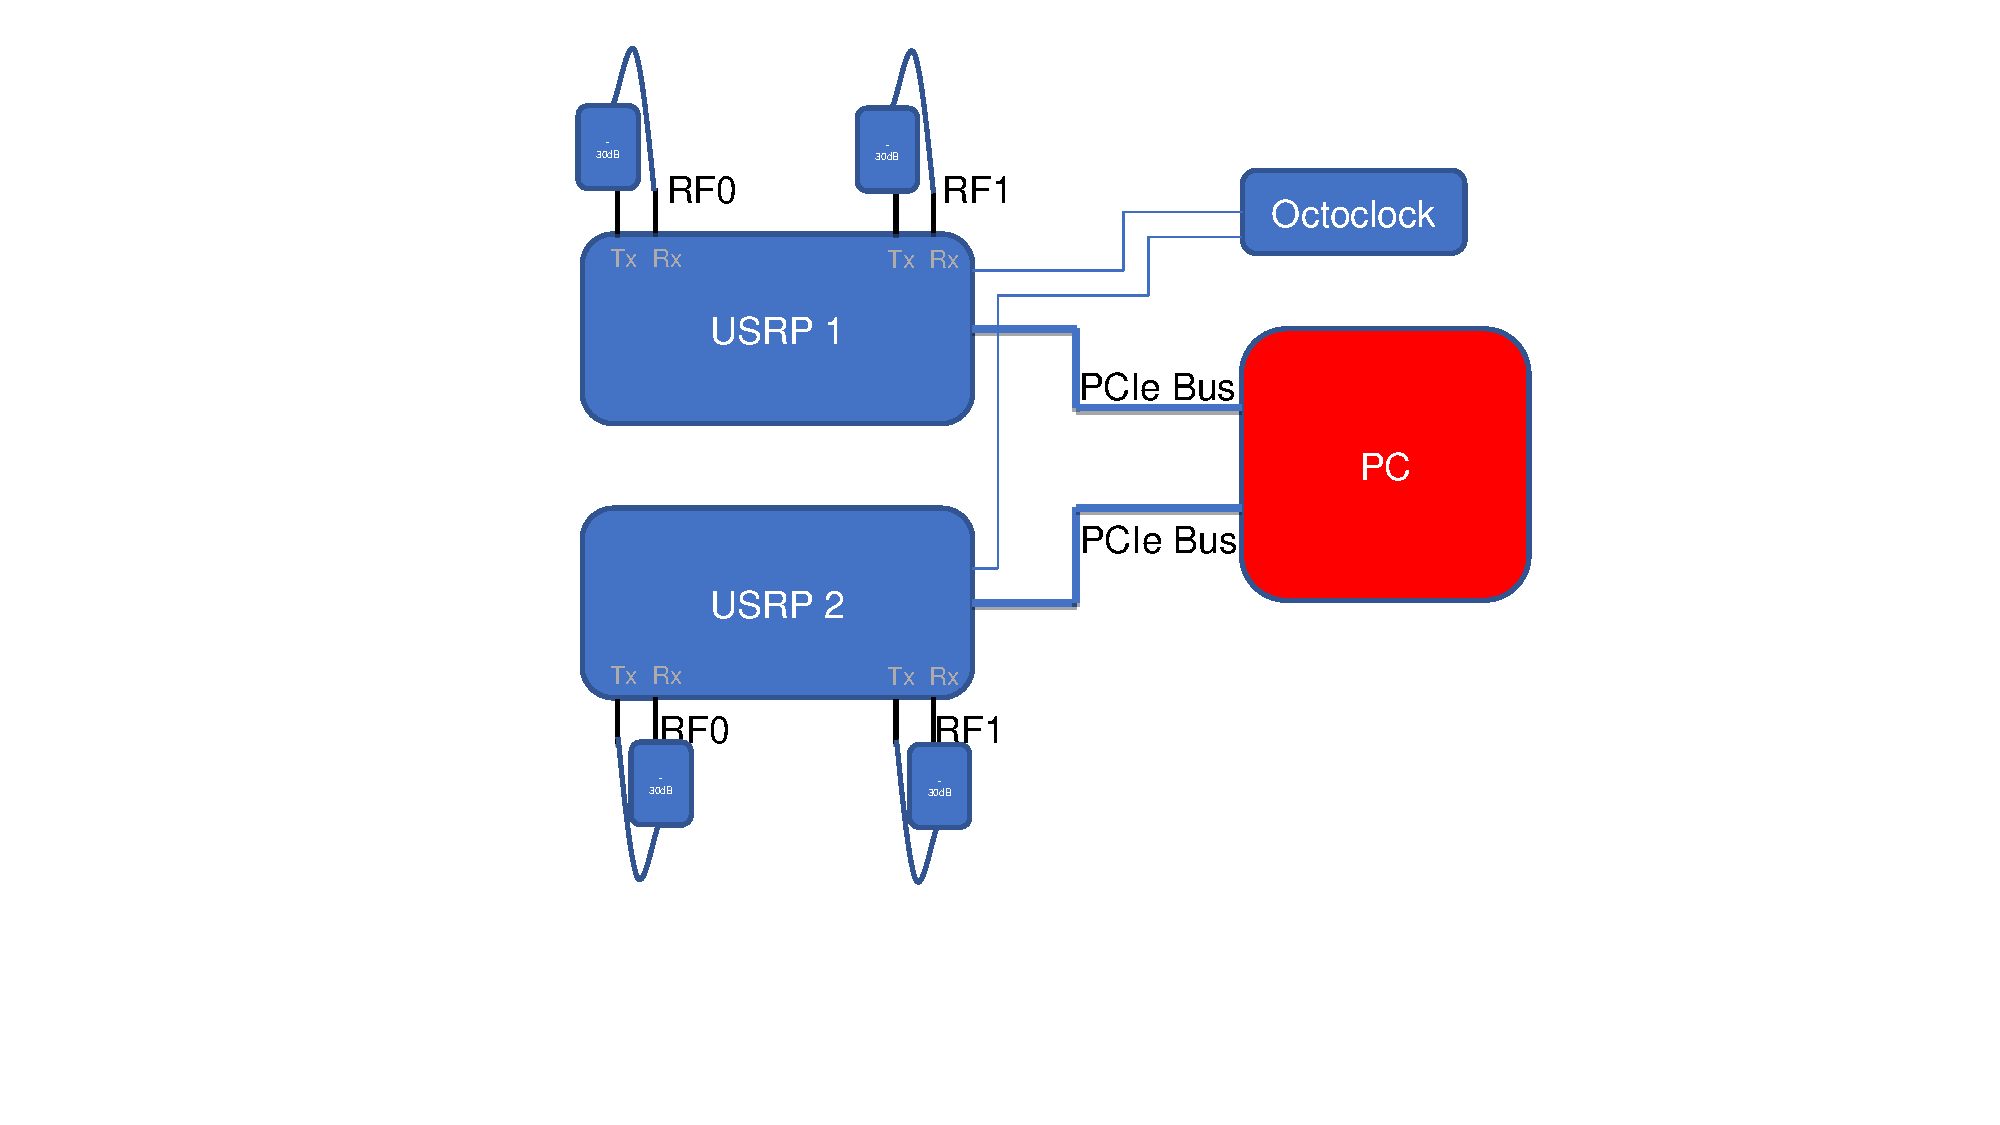
\includegraphics[width=0.9\linewidth]{../images/SetUpIllustration.pdf}
        \caption{Setup of the USRPs in loopback Configuration}
        \label{fig:SyncFail2Ch}%
    \end{figure}
\end{frame}

\begin{frame}{Option 1 - Standalone USRP}
    \begin{figure}[H]
        \centering
        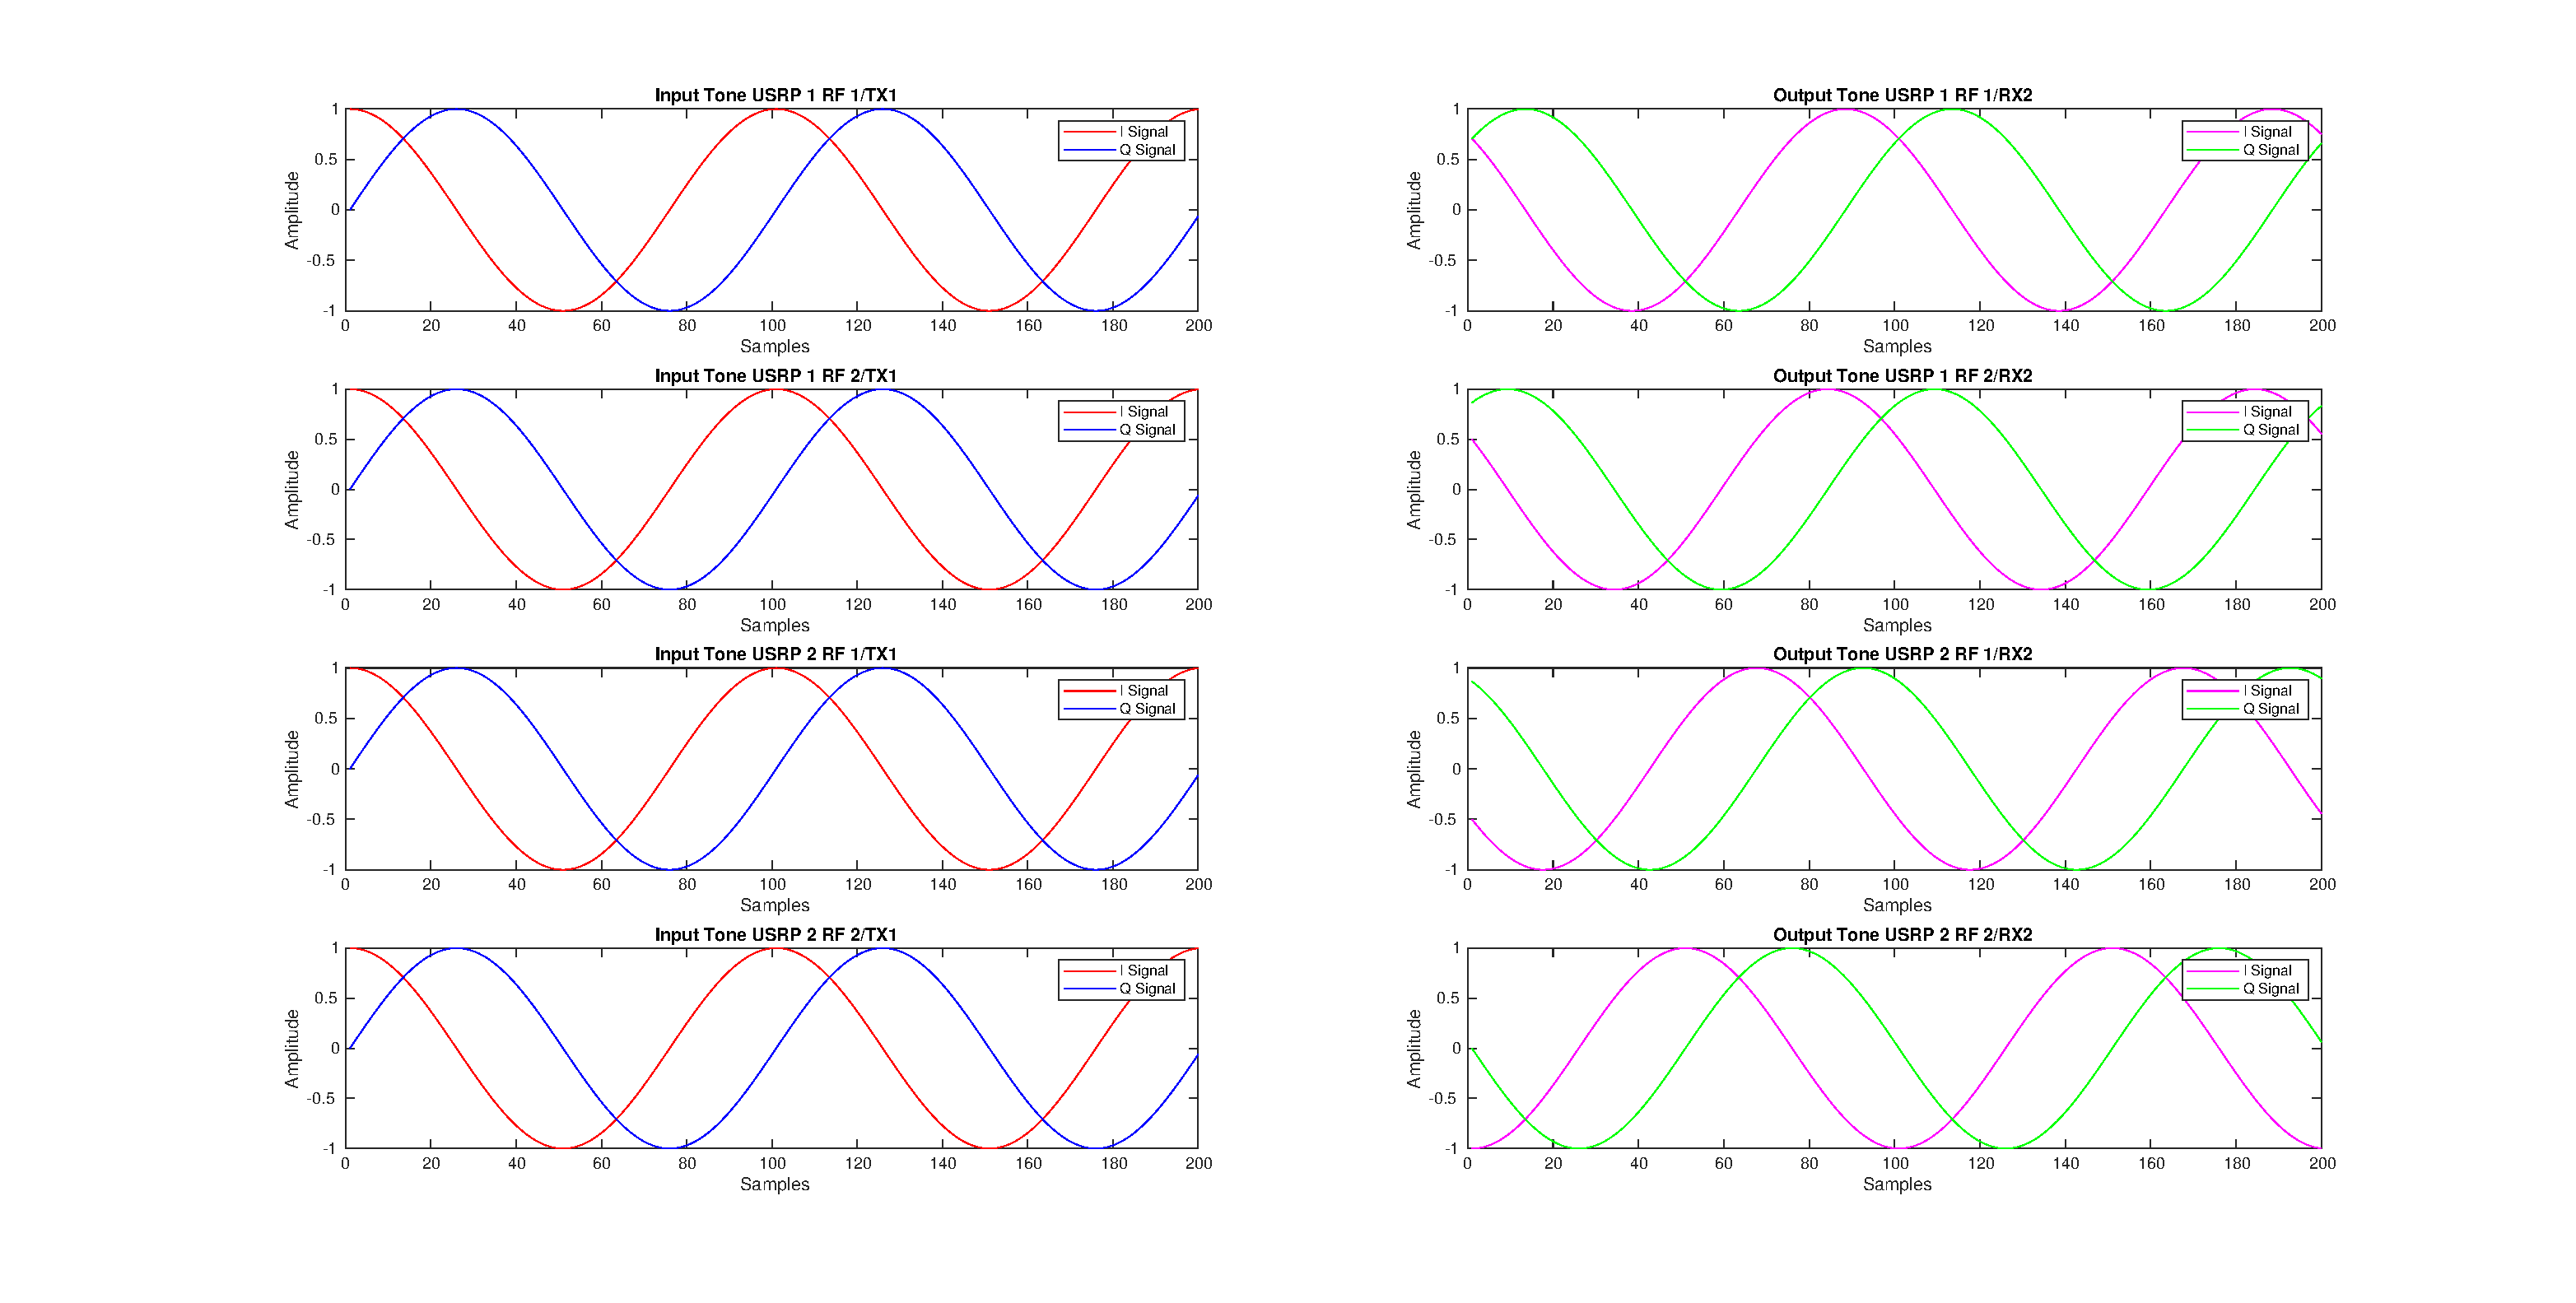
\includegraphics[width=\linewidth]{../images/SyncIssues.eps}
        \caption{The left waveforms are the TX waveforms and the right waveforms are the RX waveforms. It can be seen that the received IQ waveforms are unsynchronised and clearly have a phase shift}
        \label{fig:SyncFail2Ch}%
    \end{figure}
\end{frame}

\begin{frame}{Option 1 - Standalone USRP}
    \begin{figure}[H]
        \centering
        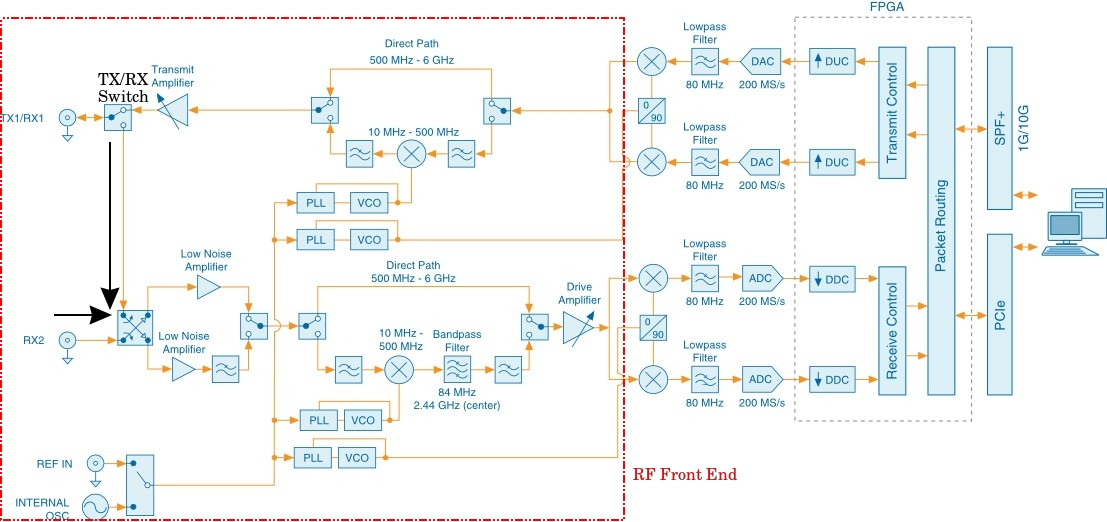
\includegraphics[width=\linewidth]{../images/USRPInternalsEdited.jpeg}
        \caption{USRP 2940 Internal Components}%
        \label{fig:USRPInternals}%
    \end{figure}
\end{frame}

\begin{frame}{Option 2 - MIMO Application Framework}
    \begin{itemize}
        \item Multi-User MIMO \textbf{Single BS} with up to 128 Antennas and up to 12 single antenna Mobile Stations (MS)
        \item Single-user MIMO transmission between one BS with up to 128 antennas and one MS with up to 12 antennas
        \item Scalable number of antennas (multi-antenna MS: between 2 and 12; BS: between 2 and 128).% Interfaces and configuration adapt automatically
        \item Modulation Schemes - QPSK to 256 QAM
        \item Automatic gain control (AGC) at the BS and MS
            \pause
        \item FPGA based real time signal processing such as 
            \begin{itemize}
                \item Modulation
                \item Over-the-air synchronization
                \item MIMO equalization
                \item MIMO precoding
            \end{itemize}
        \item Fully reconfigurable LTE like radio frame structure
        \item Bi Directional TDD and FDD functionality transmission of 20\si{\mega\hertz} bandwidth
    \end{itemize}
\end{frame}

\begin{frame}{Option 2 - MIMO Application Framework}
    \begin{table}[H]
        \begin{center}
            \resizebox{5cm}{!}{
            \begin{tabular}{|l|l|}
                \hline
                \textbf{Part Number} & \textbf{Description}          \\ \hline
                USRP-2940            & SDR                           \\ \hline
                PXIe-7976            & FPGA Module for FlexRIO       \\ \hline
                CDA-2990             & Clock Distribution Device     \\ \hline
                CPS-8910             & Switch Device for PCI Express \\ \hline
                PXIe-6674T           & Synchronization Module        \\ \hline
                PXIe-1085            & Chassis                       \\ \hline
                PXIe-8135            & Controller                    \\ \hline
            \end{tabular}
        }
        \end{center}
        \caption{Additional Hardware for required for MIMO AFW to function}
        \label{tb:MIMOAFWPartsList}
    \end{table}

    \begin{table}[h]\footnotesize
        \begin{center}
            \resizebox{10cm}{!}{
            \begin{tabular}{|l|c|c|c|c|c|}
                \hline
                \textbf{}                                                                                            & \textbf{\begin{tabular}[c]{@{}c@{}}128-antenna BS\\ 8 subsystems\end{tabular}} & \textbf{\begin{tabular}[c]{@{}c@{}}64-antenna BS\\ 4 subsystems\end{tabular}} & \textbf{\begin{tabular}[c]{@{}c@{}}32-antenna BS\\ 2 subsystems\end{tabular}} & \textbf{\begin{tabular}[c]{@{}c@{}}16-antenna BS\\ 1 subsystems\end{tabular}} & \textbf{\begin{tabular}[c]{@{}c@{}}8-antenna BS\\ 1 subsystems\end{tabular}} \\ \hline
                    \begin{tabular}[c]{@{}l@{}}USRP-29xx SDR \\ Reconfigurable Device\end{tabular}                       & 64                                                                             & 32                                                                            & 16                                                                            & 8                                                                             & 6                                                                            \\ \hline
                        \begin{tabular}[c]{@{}l@{}}PXIe-1085 Chassis \\ (18-Slot, 24 GB/sSystem Bandwidth (BW))\end{tabular} & 1                                                                              & 1                                                                             & 1                                                                             & 1                                                                             & 1                                                                            \\ \hline
                            PXIe-8135 Controller                                                                                 & 1                                                                              & 1                                                                             & 1                                                                             & 1                                                                             & 1                                                                            \\ \hline
                            PXIe-7976 FPGA Module for FlexRIO                                                                    & 5                                                                              & 3                                                                             & 2                                                                             & 2                                                                             & 2                                                                            \\ \hline
                            PXIe-6674T Synchronization                                                                           & 1                                                                              & 1                                                                             & 1                                                                             & 1                                                                             & 1                                                                            \\ \hline
                            CDA-2990 Clock Distribution Device                                                                   & 8                                                                              & 5                                                                             & 3                                                                             & 1                                                                             & 1                                                                            \\ \hline
                            CPS-8910 Switch Device for PCI Express                                                               & 8                                                                              & 4                                                                             & 2                                                                             & 1                                                                             & 1                                                                            \\ \hline
            \end{tabular}
            }
            \caption{MIMO Configurations and HW requirements}
            \label{tb:MIMOAFWConf}
        \end{center}
    \end{table}
\end{frame}

\begin{frame}{Option 2 - MIMO Application Framework}
    \begin{figure}[H]
        \centering
        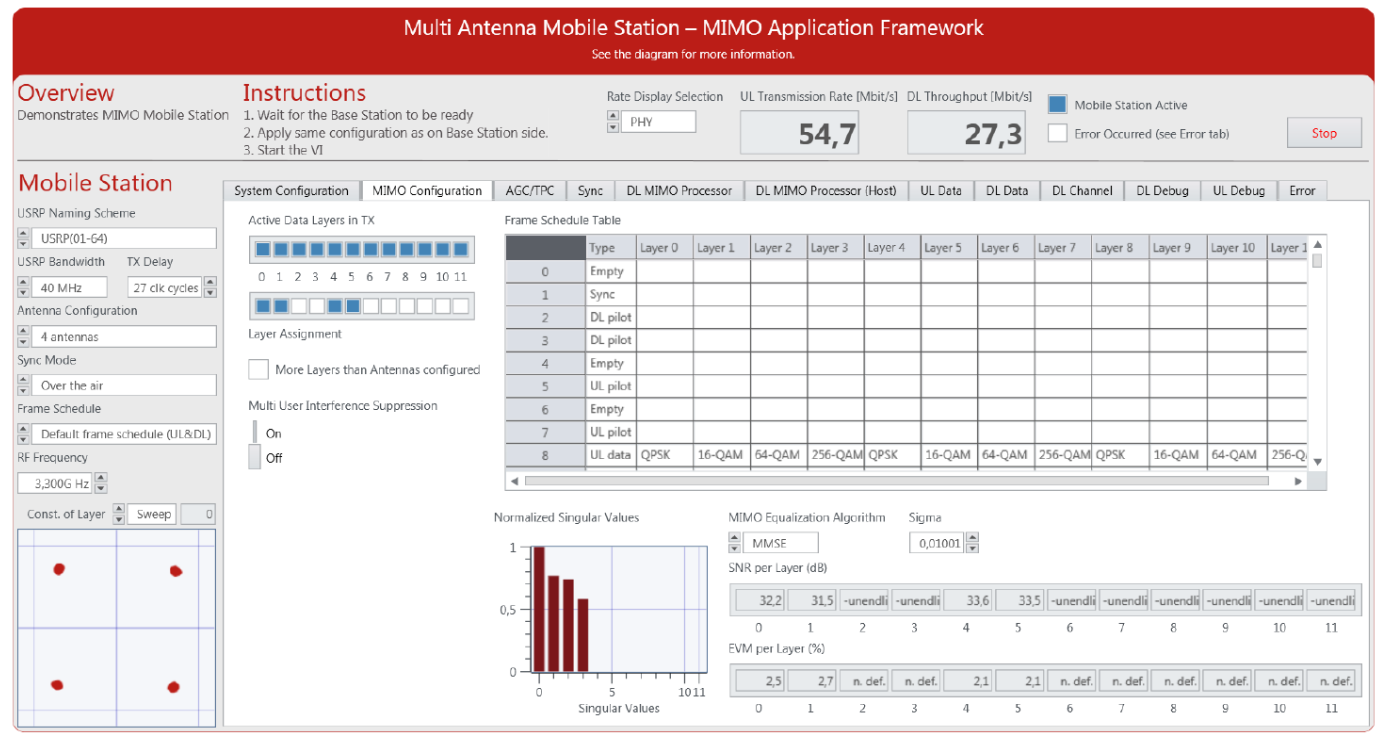
\includegraphics[width=\linewidth]{../images/MIMOAFWScreen.png}
        \caption{MIMO AFW}
    \end{figure}
\end{frame}

\begin{frame}{Option 3 - LTE Application Framework MIMO Extension}
    \begin{itemize}
        \item Based on a LTE Application Framework, an LTE Release 10 implementation
            \bigskip
        \item Developed by NI to demonstrate a functioning 2x2 MIMO System
            \bigskip
        \item Provides a \textbf{Downlink ONLY} 2x2 LTE Setup
            \bigskip
        \item Upto 64 QAM modulation
            \bigskip
        \item FPGA based realtime signal processing
            \bigskip
        \item 3 different Equalisation algorithms
            \begin{itemize}
                \item Matched Filter
                \item Zero Forcing
                \item MMSE
            \end{itemize}
    \end{itemize}
\end{frame}

\begin{frame}{LTE Fundamentals}
    \begin{itemize}
        \item OFDMA based physical layer
            \bigskip
        \item Frame based communication scheme of 10\si{\milli\second} per Frame
            \bigskip
            \pause
        \item Each frame subdivided into 10 Subframes
            \pause
            \bigskip
        \item Each subframe has 14 Symbols
            \pause
            \bigskip
        \item Contain many different signals
            \begin{itemize}
                \item \alert<+>{Primary Synchronisation Signal (PSS) -\textbf{QPSK}}
                \item \alert<+>{Secondary Synchronisation Signal (SSS) - \textbf{BPSK}}
                \item \alert<+>{Cell Specific Reference Signal (CRS) - \textbf{QPSK}}
            \end{itemize}
    \end{itemize}
\end{frame}


\begin{frame}{LTE Fundamentals}
    \begin{figure}[H]
        \begin{center}
            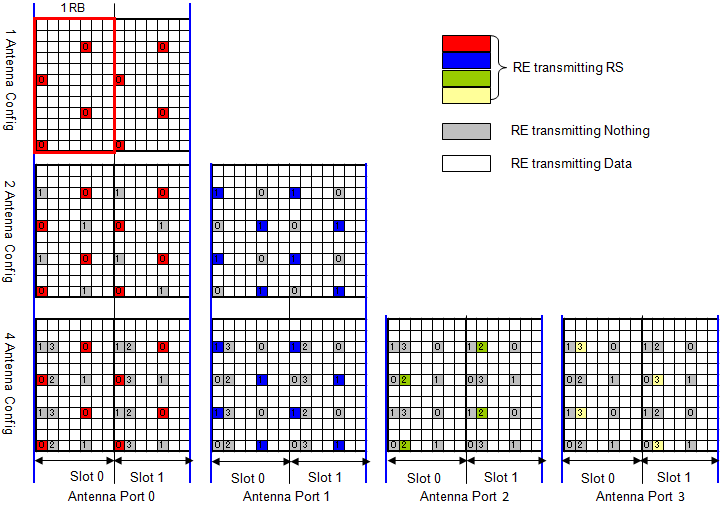
\includegraphics[width=0.75\linewidth]{../images/CRSMultiAntenna.png}
            \caption{Cell Reference Signal layout for multi antenna configurations of 1,2 and 4 antenna systems in LTE}
            \label{fig:CRSMultiAntenna}
        \end{center}
    \end{figure}
\end{frame}

\begin{frame}{Experimental Setup - FPGA}
\end{frame}

\begin{frame}{Experimental Setup - CRS Data Transmission}
    \begin{figure}%
        \centering
        \subfloat[Channel Estimation Interpolation over Frequency]{{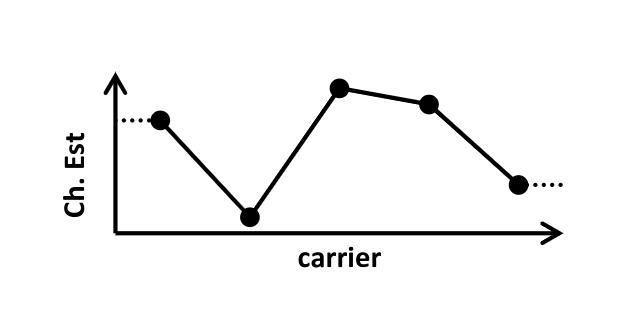
\includegraphics[width=0.35\linewidth]{../images/ChEstInterpolation.png} }}%
        \qquad
        \subfloat[Channel Estimation Zero order hold over time]{{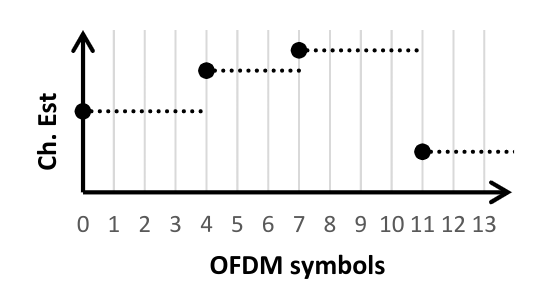
\includegraphics[width=0.35\linewidth]{../images/ChEstZOH.png} }}%
        \caption{Illustration of channel estimation interpolation over time and frequency}%
    \end{figure}

    \pause
    \begin{itemize}
        \item The RF Front end phase offset correction is applied to all the subcarriers and time symbols
        \item Fixed transmit pattern as defined by standard
    \end{itemize}
\end{frame}

\begin{frame}{Experimental Setup - Wideband Noise Calculation}
\end{frame}

\begin{frame}{\huge Demo}
\end{frame}

\begin{frame}[fragile]{Results - Data Loss}
    \begin{lstlisting}[style=DOS,basicstyle=\fontsize{5}{6}\selectfont]
    Microsoft Windows [Version 10.0.18363.1016]
    (c) 2019 Microsoft Corporation. Alle Rechte vorbehalten.

    C:\Users\ge69mog>cd Downloads\iperf-2.0.9-win64\iperf-2.0.9-win64

    C:\Users\ge69mog\Downloads\iperf-2.0.9-win64\iperf-2.0.9-win64>iperf.exe -s -u
    -B 127.0.0.1 -i 1 -p 60000
    ------------------------------------------------------------
    Server listening on UDP port 60000
    Binding to local address 127.0.0.1
    Receiving 1470 byte datagrams
    UDP buffer size:  208 KByte (default)
    ------------------------------------------------------------
    [  3] local 127.0.0.1 port 60000 connected with 127.0.0.1 port 49721
    [ ID] Interval       Transfer     Bandwidth        Jitter   Lost/Total Datagrams
    [  3]  0.0- 1.0 sec   996 KBytes  8.16 Mbits/sec   2.017 ms  166/  860 ((*@\textcolor{red}{19\%}@*))
    [  3] 0.00-1.00 sec  50 datagrams received out-of-order
    [  3]  1.0- 2.0 sec   904 KBytes  7.41 Mbits/sec   2.426 ms  227/  857 ((*@\textcolor{red}{26\%}@*))
    [  3] 1.00-2.00 sec  70 datagrams received out-of-order
    [  3]  2.0- 3.0 sec   902 KBytes  7.39 Mbits/sec   2.148 ms  219/  847 ((*@\textcolor{red}{26\%}@*))
    [  3] 2.00-3.00 sec  61 datagrams received out-of-order
    [  3]  3.0- 4.0 sec   916 KBytes  7.50 Mbits/sec   1.904 ms  222/  860 ((*@\textcolor{red}{26\%}@*))
    [  3] 3.00-4.00 sec  69 datagrams received out-of-order
    [  3]  4.0- 5.0 sec   871 KBytes  7.14 Mbits/sec   4.137 ms  206/  813 ((*@\textcolor{red}{25\%}@*))
    [  3] 4.00-5.00 sec  56 datagrams received out-of-order
    [  3]  5.0- 6.0 sec   953 KBytes  7.81 Mbits/sec   4.710 ms  226/  890 ((*@\textcolor{red}{25\%}@*))
    [  3] 5.00-6.00 sec  86 datagrams received out-of-order
    [  3]  6.0- 7.0 sec   828 KBytes  6.79 Mbits/sec   2.786 ms  253/  830 ((*@\textcolor{red}{30\%}@*))
    [  3] 6.00-7.00 sec  84 datagrams received out-of-order
    [  3]  7.0- 8.0 sec   843 KBytes  6.90 Mbits/sec   4.467 ms  250/  837 ((*@\textcolor{red}{30\%}@*))
    [  3] 7.00-8.00 sec  90 datagrams received out-of-order
    [  3]  8.0- 9.0 sec   970 KBytes  7.95 Mbits/sec   1.648 ms  200/  876 ((*@\textcolor{red}{23\%}@*))
    [  3] 8.00-9.00 sec  61 datagrams received out-of-order
    [  3]  0.0-10.0 sec  8.86 MBytes  7.43 Mbits/sec   2.888 ms 2183/ 8505 ((*@\textcolor{red}{26\%}@*))
    [  3] 0.00-10.00 sec  689 datagrams received out-of-order
    \end{lstlisting}
\end{frame}

\begin{frame}{Results - CRS Data Transmission}
    \begin{figure}[!htb]
        \centering
        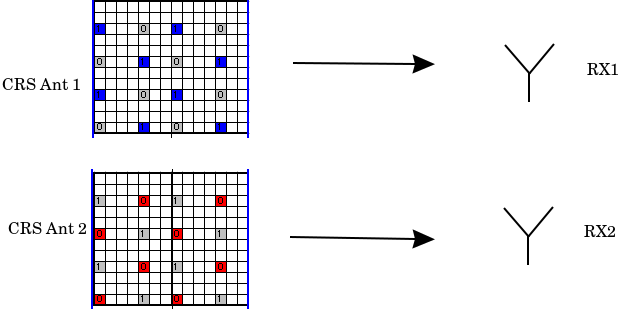
\includegraphics[width=0.8\linewidth]{../images/MultiAntennaCRSXYPairEdited.png}
        \caption{Illustration of the CRS signals and channel estimation coefficients used as the ($x$,$y$) pair}
    \end{figure}
    \begin{itemize}
        \item A sequence of 8342 time symbols for the 200 CRS carriers were recorded
        \item Final matrix size of $200\times8342$
    \end{itemize}
\end{frame}

\begin{frame}{Results - INN Detection}

    \begin{figure}%
        \centering
        \subfloat[XY plot of the real parts of the input signals $x_1$ and $x_2$ with noise]{{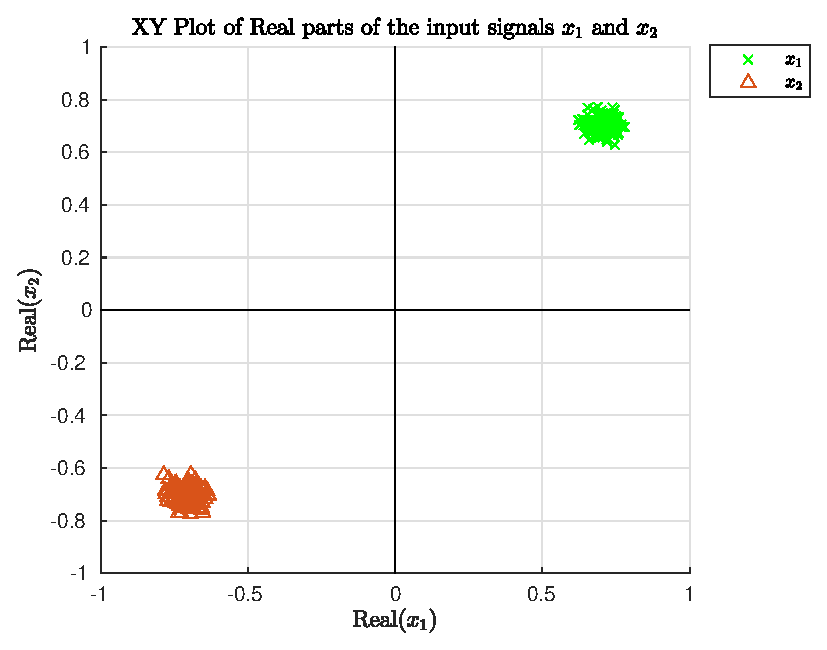
\includegraphics[width=0.45\linewidth]{../images/INNxn.eps} }}%
        \qquad
        \subfloat[XY plot of the real parts of the INN Estimated signals $\hat{x_1}$ and $\hat{x_2}$]{{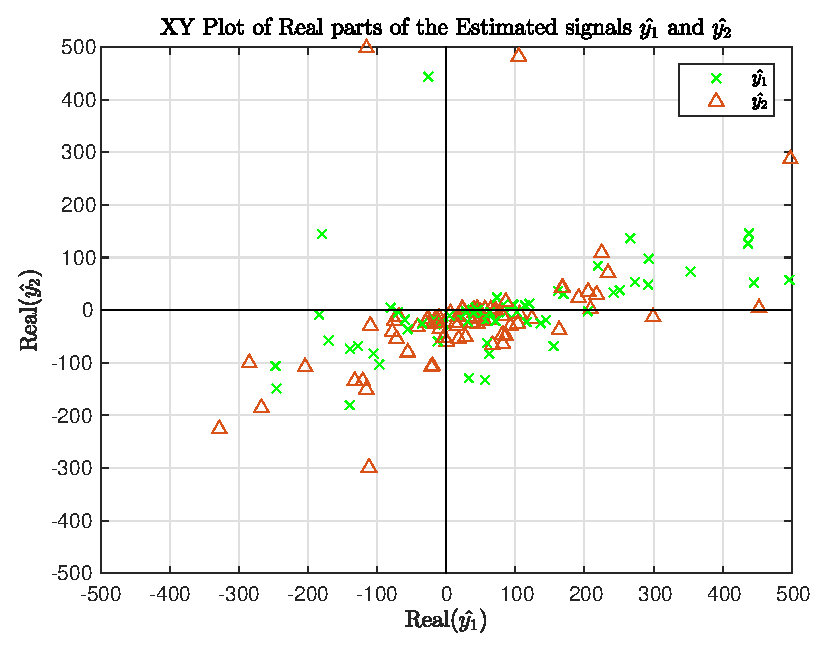
\includegraphics[width=0.45\linewidth]{../images/INNResult.eps} }}%
        \caption{Detection accuracy of \textbf{22\%} from the INN}
    \end{figure}
\end{frame}

\begin{frame}{Conclusion}
\end{frame}

\begin{frame}[allowframebreaks]{References}
    \begin{columns}
        \column{0.80\paperwidth}
        \printbibliography
    \end{columns}
\end{frame}

{
    \begin{frame}{A Slide with a different header}
        Some text, possibly \textbf{bold} or \alert{highlighted}.

        \begin{itemize}
            \item Bullet points
            \item Second point
                \begin{itemize}
                    \item Sub-bullet
                \end{itemize}
        \end{itemize}

        \pause
        \begin{enumerate}
            \item First
            \item Second
            \item Third
        \end{enumerate}

    \end{frame}
}

{\lowertitle\lowertitle
\setbeamertemplate{headline}[msvtum]
\begin{frame}{Frame with highlight boxes and alternative header}

    \begin{block}{Important Result\footnotemark[1]}
        The following holds:\footnotemark[2]
        \begin{equation*}
            E = mc^2
        \end{equation*}
    \end{block}
    \footnotetext[1]{This is a footnote in a block title.}
    \footnotetext[2]{This is a footnote in a block body.}

    \pause

    \begin{center}
        $\Downarrow$
    \end{center}

    \begin{alertblock}{}
        Can also be used without a title.
        Three color types are available: block (blue), alertblock (red), and exampleblock (green).
        Spacing may need some manual adjustment if formulas are included at the top or bottom of blocks.
    \end{alertblock}

\end{frame}
}

{
    \setbeamertemplate{headline}[no]
    \begin{frame}{Some math}
        \begin{itemize}
            \item We consider some simple formulas, e.g. $\max(0,1) = 1$
            \item Complicated formula: $h_J(y) = \sum_{K\subset N}\int_{\mathbb{R}}g_K(x,y)f_J(x)dx$
            \item This looks slightly weired since math fonts are smaller than text fonts.
        \end{itemize}

        However, this does not really affect equations.
        \begin{equation*}
            h_J(y) = \sum_{K\subset N}\int_{\mathbb{R}}g_K(x,y)f_J(x)dx
        \end{equation*}
    \end{frame}
}

\begin{frame}{}
    No title on this frame.\footnote{Smith et al., 2100: ``Title of a paper that will be written in the future'', \itshape IEEE Trans Inf. Theory}

    \begin{exampleblock}{Example Block}
        Spacing around blocks is minimal (if option frameblock is used).
        Extra spaces, e.g. \texttt{vskip} or \texttt{vspace}, should be used.
    \end{exampleblock}

    Text below block.

\end{frame}


\section{Main Part}


\begin{frame}{TUM Colors}
    In diagrams and plots only use the following colors:
    \begin{itemize}
        \item Black, White
        \item \textcolor{TUMBeamerYellow}{Yellow, RGB 255/180/000}
        \item \textcolor{TUMBeamerOrange}{Orange, RGB 255/128/000}
        \item \textcolor{TUMBeamerRed}{Red, RGB 229/052/024}
        \item \textcolor{TUMBeamerDarkRed}{Dark Red, RGB 202/033/063}
        \item \textcolor{TUMBeamerBlue}{Blue, RGB 000/153/255}
        \item \textcolor{TUMBeamerLightBlue}{Light Blue, RGB 065/190/255}
        \item \textcolor{TUMBeamerGreen}{Green, RGB 145/172/107}
        \item \textcolor{TUMBeamerLightGreen}{Light Green, RGB 181/202/130}
    \end{itemize}
\end{frame}



\section{Conclusion}


\begin{frame}{Final Slide}
    Add some vertical space.

    \vspace{8mm}
    Increase spacing between bullet points:

    \vspace{5mm}
\begin{itemize}\addtolength{\itemsep}{5mm}
        \item More information can be found in the \alert{beamer user guide}
        \item Use \texttt{pdflatex} to compile the source
        \item Have fun creating your slides!
\end{itemize}
\end{frame}


\end{document}
